\documentclass[11pt, a4paper]{article}

\usepackage[left=2cm,text={17cm, 24cm},top=3cm]{geometry}
\usepackage[czech]{babel}
\usepackage[IL2]{fontenc}
\usepackage[utf8]{inputenc}
\usepackage{times}
\usepackage{url}
\usepackage{multirow}
\usepackage{amsmath}
\usepackage{graphicx}
\usepackage{float}
\usepackage{lscape}
\usepackage[linesnumbered,lined,ruled,czech]{algorithm2e}

\def \noteA {Kdyby byl problém s~\texttt{cline}, zkuste se podívat třeba sem: \urlstyle{rm}\url{http://www.abclinuxu.cz/tex/poradna/show/325037}.}

\def \noteB {Pro nápovědu, jak zacházet s~prostředím\texttt{ algorithm}, můžeme zkusit tuhle stránku:\\
\urlstyle{rm}\url{http://ftp.cstug.cz/pub/tex/CTAN/macros/latex/contrib/algorithms/algorithms.pdf}.}

\def \noteC {Pro\texttt{ algorithm2e }zase tuhle:
\urlstyle{rm}\url{http://ftp.cstug.cz/pub/tex/CTAN/macros/latex/contrib/algorithm2e/doc/algorithm2e.pdf}.}

\begin{document}
\begin{titlepage}
    \begin{center}
        \Huge{\textsc{Vysoké učení technické v~Brně}}\\
        \huge{\textsc{Fakulta informačních technologií}}\\
        \vspace{\stretch{0.382}}
        \LARGE{Typografie a publikování -- 3. projekt}\\
        \Huge{Tabulky a obrázky}\\
        \vspace{\stretch{0.618}}
    \end{center}
    {\Large \today \hfill Alexandr Chalupnik (xchalu15)}
\end{titlepage}

\section{Úvodní strana}
Název práce umístěte do zlatého řezu a nezapomeňte uvést dnešní datum a vaše jméno a příjmení.
\section{Tabulky}
Pro sázení tabulek můžeme použít buď prostředí\verb| tabbing |nebo prostředí\verb| tabular|.
\subsection{Prostředí\texttt{ tabbing}}
Při použití\verb| tabbing |vypadá tabulka následovně:

\begin{tabbing}
Vodní meloun\qquad \= 32,--\qquad \= 1\,kus \kill
\bfseries Ovoce \>
\bfseries Cena \>
\bfseries Množství \\
Jablka \> 25,90 \> 3\,kg \\
Hrušky \> 27,40 \> 2,5\,kg \\
Vodní meloun \> 35,-- \> 1\,kus \\
\end{tabbing}

\noindent Toto prostředí se dá také použít pro sázení algoritmů, ovšem vhodnější je použít prostředí\verb| algorithm |nebo \verb|algorithm2e |(viz sekce \ref{algo}).


\subsection{Prostředí\texttt{ tabbular}}
Další možností, jak vytvořit tabulku, je použít prostředí\verb| tabular|. Tabulky pak budou vypadat takto\footnote{\noteA}:

\begin{table}[h!] \catcode`\-=12
\centering
    \begin{tabular}{|l|c|c|}\hline
         & \multicolumn{2}{c|}{\bfseries Cena} \\ \cline{2-3}
         \bfseries Měna &
         \bfseries nákup &
         \bfseries prodej \\ \hline
         EUR & 25,475 & 27,045\\
         GBP & 28,835 & 30,705\\
         USD & 22,943 & 24,357\\ \hline
    \end{tabular}
    \caption{Tabulka kurzů k~dnešnímu dni} \label{tab:kurzy}
\end{table}

\begin{table}[h!] \catcode`\-=12
\centering
    \begin{tabular}{|c|c|}\hline
         $A$ &
         $\neg A$ \\ \hline
         \bfseries P & N \\ \hline
         \bfseries O~& O~\\ \hline
         \bfseries X & X \\ \hline
         \bfseries N & P \\ \hline
    \end{tabular}
    \begin{tabular}{|c|c|c|c|c|c|}\hline
        \multicolumn{2}{|c|}{\multirow{2}{*}{$A \land B$}} & \multicolumn{4}{c|}{$B$}\\ \cline{3-6} 
        \multicolumn{2}{|c|}{} & \textbf{P} & \textbf{O} & \textbf{X} & \textbf{N} \\ \hline
        \multirow{4}{*}{$A$} & \textbf{P} & P & O~& X & N \\ \cline{2-6} 
                             & \textbf{O} & O~& O~& N & N \\ \cline{2-6} 
                             & \textbf{X} & X & N & X & N \\ \cline{2-6} 
                             & \textbf{N} & N & N & N & N \\ \hline
    \end{tabular}
    \begin{tabular}{|c|c|c|c|c|c|}\hline
        \multicolumn{2}{|c|}{\multirow{2}{*}{$A \lor B$}} & \multicolumn{4}{c|}{$B$}\\ \cline{3-6} 
        \multicolumn{2}{|c|}{} & \textbf{P} & \textbf{O} & \textbf{X} & \textbf{N} \\ \hline
        \multirow{4}{*}{$A$} & \textbf{P} & P & P & P & P \\ \cline{2-6} 
                             & \textbf{O} & P & O~& P & O~\\ \cline{2-6} 
                             & \textbf{X} & P & P & X & X \\ \cline{2-6} 
                             & \textbf{N} & P & O~& X & N \\ \hline
    \end{tabular}
    \begin{tabular}{|c|c|c|c|c|c|}\hline
        \multicolumn{2}{|c|}{\multirow{2}{*}{$A \to B$}} & \multicolumn{4}{c|}{$B$}\\ \cline{3-6} 
        \multicolumn{2}{|c|}{} & \textbf{P} & \textbf{O} & \textbf{X} & \textbf{N} \\ \hline
        \multirow{4}{*}{$A$} & \textbf{P} & P & O~& X & N \\ \cline{2-6} 
                             & \textbf{O} & P & O~& P & O~\\ \cline{2-6} 
                             & \textbf{X} & P & P & X & X \\ \cline{2-6} 
                             & \textbf{N} & P & P & P & P \\ \hline
    \end{tabular}
    
    
    \caption{Protože Kleeneho trojhodnotová logika už je \uv{zastaralá}, uvádíme si zde příklad čtyřhodnotové logiky} \label{tab:logika}
\end{table}

\pagebreak

\section{Algoritmy} \label{algo}
Pokud budeme chtít vysázet algoritmus, můžeme použít prostředí\verb| algorithm|\footnote{\noteB} nebo\verb| algorithm2e|\footnote{\noteC}. Příklad~použití prostředí\verb| algorithm2e |viz Algoritmus \ref{algo:alg1}.
\vspace{2em}

\begin{algorithm}[H]
    \label{algo:alg1}
    \caption{\textsc{FastSLAM}}
    \SetNlSty{textrm}{}{:}
    \DontPrintSemicolon
    \SetAlgoNoLine
    \SetNlSkip{-1em}
    \SetKwFor{For}{for}{do}{end~for}
    \KwIn{$(X_{t-1},u_t,z_t)$}
    \KwOut{$X_t$}
    \BlankLine
\Indp\Indpp
$ \overline{X_t} = X_t = 0 $ \\
    \For{$k = 1$ \upshape{to} $M$}{
        $x_t^{[k]} = \emph{sample\_motion\_model}(u_t, x^{[k]}_{t-1})$\;
        $w_t^{[k]} = \emph{measurement\_model}(z_t, x^{[k]}_t, m_{t-1})$\;
        $m_t^{[k]} = updated\_occupancy\_grid(z_t, x_t^{[k]}, m_{t-1}^{[k]})$\;
        $\overline{X_t} = \overline{X_t} + \langle x_x^{[m]}, w_t^{[m]} \rangle $\;
        }
    \For {$k = 1$ \upshape{to} $M$}{
        draw $i$ with probability $\approx w_t^{[i]}$\;
        add $\langle x_x^{[k]}, m_t^{[k]} \rangle$ to $X_t$\;
        }
    \KwRet{$X_t$}
\end{algorithm}

\section{Obrázky}
Do našich článků můžeme samozřejmě vkládat obrázky. Pokud je obrázek fotografie, můžeme klidně použít bitmapový soubor. Pokud by to ale mělo být nějaké schéma nebo něco podobného, je dobrým zvykem takovýto obrázek vytvořit vektorově.

\begin{figure}[H]
    \centering
    \scalebox{0.40}{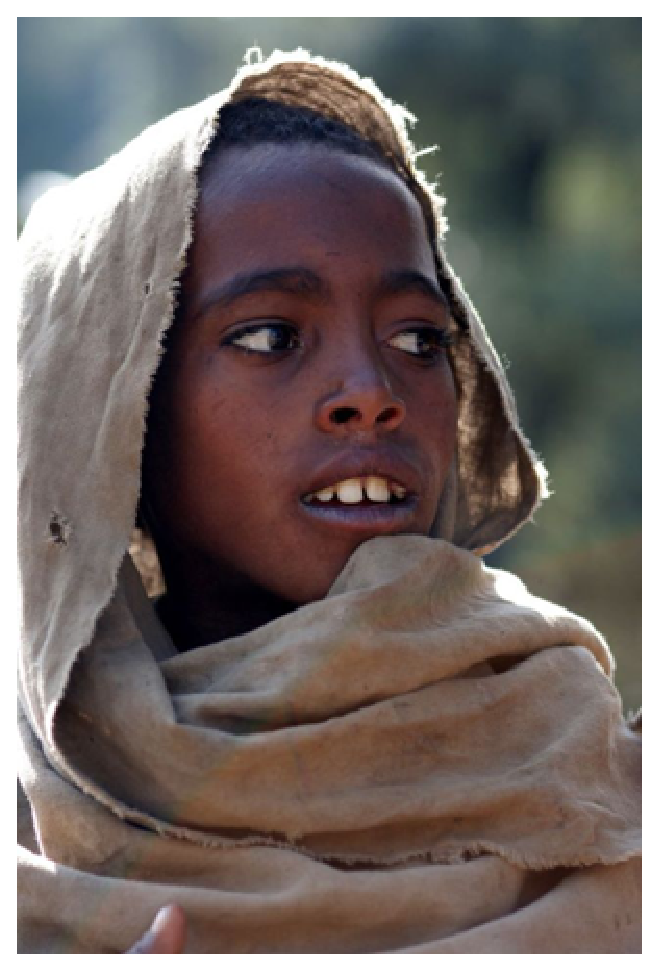
\includegraphics{etiopan.eps}\hspace{0.5em}\reflectbox{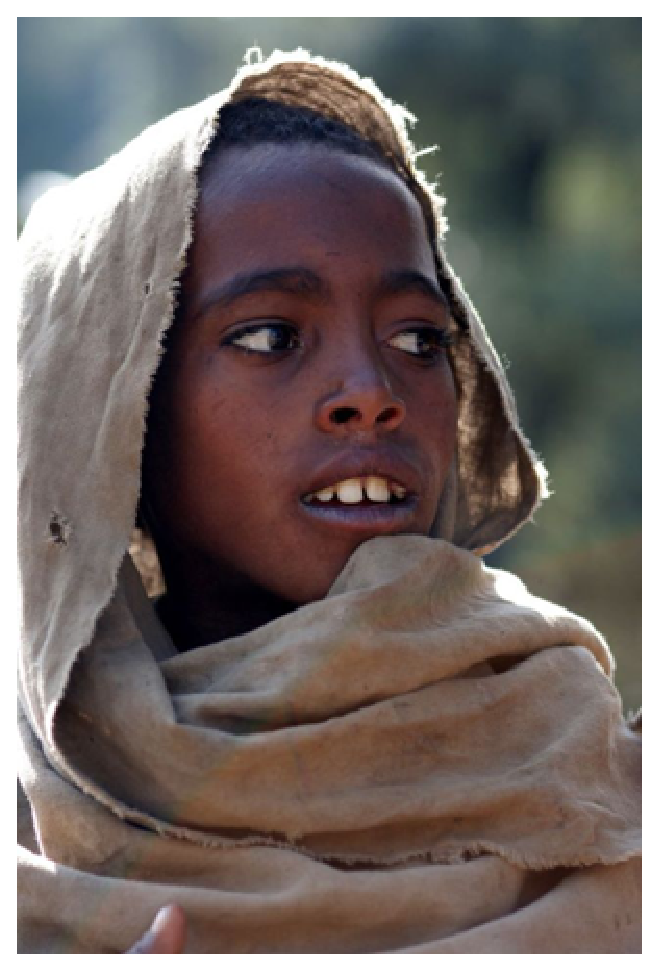
\includegraphics{etiopan.eps}}}
    \caption{Malý Etiopánek a jeho bratříček}
    \label{fig:etiopan}
\end{figure}

\newpage

Rozdíl mezi vektorovým\dots
\begin{figure}[H]
    \centering
    \scalebox{0.40}{
\includegraphics{oniisan.eps}}
    \caption{Vektorový obrázek}
    \label{fig:vector}
\end{figure}
\medskip
\dots a bitmapovým obrázkem
\begin{figure}[H]
    \centering
    \scalebox{0.65}{
\includegraphics{oniisan2.eps}}
    \caption{Bitmapový obrázek}
    \label{fig:bitmap}
\end{figure}
\bigskip
se projeví například při zvětšení.

Odkazy (nejen ty) na obrázky \ref{fig:etiopan}, \ref{fig:vector} a \ref{fig:bitmap}, na tabulky \ref{tab:kurzy} a \ref{tab:logika} a také na algoritmus \ref{algo:alg1} jsou udělány pomocí křížových odkazů. Pak je ovšem potřeba zdrojový soubor přeložit dvakrát.

Vektorové obrázky lze vytvořit přímo v~\LaTeX{}u, například pomocí prostředí\verb| picture|.

\newpage

\begin{landscape}

\begin{figure}[H]
    \centering
    \setlength{\unitlength}{1mm}
    \begin{picture}(200,110)
    
        %ramecek
        \linethickness{0.4mm}
        \put(0,0){\framebox(200, 99){}}
        %kruh
        \put(170,80){\circle{14}}
        
        %levy obdelnik
        \multiput(70,45)(55,0){2}{\line(0,1){10}}
        \multiput(70,45)(0,10){2}{\line(1,0){55}}
        
        %pravy obdelnik
        \multiput(125,45)(50,0){2}{\line(0,1){2}}
        \multiput(125,45)(0,2){2}{\line(1,0){50}}
        
        %velky obdelnik
        \multiput(45,40)(140,0){2}{\line(0,1){5}}
        \multiput(45,40)(0,5){2}{\line(1,0){140}}
        \thicklines
        \put(45,40){\line(6,-5){13}}
        
        %prostredni obdelnik
        \put(85,27){\line(0,1){10}}
        \put(85,37){\line(1,0){95}}
        \put(180,21){\line(0,1){16}}
        
        %levy okraj
        \put(30,49.5){\line(1,0){40}}
        \put(30,14){\line(0,1){35.5}}
        
        %levy lichobeznik
        \put(40,14){\line(0,1){15}}
        \put(40,29){\line(1,0){40}}
        \thicklines
        \put(80,29){\line(5,-2){38}}
        
        %pravy lichobeznik
        \put(185,14){\line(0,1){7}}
        \put(100,21){\line(1,0){85}}
        
        %zem
        \linethickness{1.5mm}
        \put(5,13.5){\line(1,0){190}}

    \end{picture}
    \caption{Příklad funkcionalistické architektury}
    \label{picture:architektura}
\end{figure}
\end{landscape}




\end{document}
